\text{FIGURE 1. A 5-round differential path with probability of $2^{-58}$}

\renewcommand{\arraystretch}{1.5} % Adjust the row height
\setlength{\tabcolsep}{0pt} % Remove extra padding between columns

\begin{center}
    \resizebox{\textwidth}{!}{%
        \(
        \begin{array}{|p{0.5cm}|p{0.5cm}|p{0.5cm}|p{0.5cm}|}
            \hline
            \delta &  &  & \\ \hline
                   &  &  & \\ \hline
                   &  &  & \\ \hline
                   &  &  & \\ \hline
        \end{array}
        \hspace{2pt} % Decrease space here
        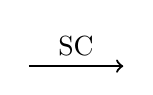
\begin{tikzpicture}[baseline={(current bounding box.center)}, scale=0.4]
            % Arrow from first grid to second grid
            \draw[->, thick] (0, 0) -- (3, 0)
            node[midway, above] {SC};
        \end{tikzpicture}
        \hspace{2pt} % Decrease space here
        \begin{array}{|p{0.5cm}|p{0.5cm}|p{0.5cm}|p{0.5cm}|}
            \hline
            A &  &  & \\ \hline
              &  &  & \\ \hline
              &  &  & \\ \hline
              &  &  & \\ \hline
        \end{array}
        \hspace{2pt} % Decrease space here
        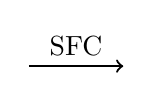
\begin{tikzpicture}[baseline={(current bounding box.center)}, scale=0.4]
            % Arrow from second grid to third grid
            \draw[->, thick] (0, 0) -- (3, 0)
            node[midway, above] {SFC};
        \end{tikzpicture}
        \hspace{2pt} % Decrease space here
        \begin{array}{|p{0.5cm}|p{0.5cm}|p{0.5cm}|p{0.5cm}|}
            \hline
            A &  &  & \\ \hline
              &  &  & \\ \hline
              &  &  & \\ \hline
              &  &  & \\ \hline
        \end{array}
        \hspace{2pt} % Decrease space here
        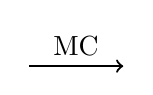
\begin{tikzpicture}[baseline={(current bounding box.center)}, scale=0.4]
            % Arrow from third grid to fourth grid
            \draw[->, thick] (0, 0) -- (3, 0)
            node[midway, above] {MC};
        \end{tikzpicture}
        \hspace{2pt} % Decrease space here
        \begin{array}{|p{0.5cm}|p{0.5cm}|p{0.5cm}|p{0.5cm}|}
            \hline
              &  &  & \\ \hline
            A &  &  & \\ \hline
            A &  &  & \\ \hline
            A &  &  & \\ \hline
        \end{array}
        \)
        \hspace{2pt} % Decrease space here

        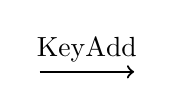
\begin{tikzpicture}[baseline={(current bounding box.center)}, scale=0.4]
            % Arrow from third grid to fourth grid
            \draw[->, thick] (0, 0) -- (3, 0)
            node[midway, above] {KeyAdd};
        \end{tikzpicture}

    }
\end{center}
\begin{center}
    \resizebox{\textwidth}{!}{%
        \(
        \begin{array}{|p{0.5cm}|p{0.5cm}|p{0.5cm}|p{0.5cm}|}
            \hline
              &  &  & \\ \hline
            A &  &  & \\ \hline
            A &  &  & \\ \hline
            A &  &  & \\ \hline
        \end{array}
        \hspace{2pt} % Decrease space here
        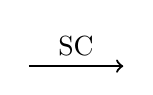
\begin{tikzpicture}[baseline={(current bounding box.center)}, scale=0.4]
            % Arrow from first grid to second grid
            \draw[->, thick] (0, 0) -- (3, 0)
            node[midway, above] {SC};
        \end{tikzpicture}
        \hspace{2pt} % Decrease space here
        \begin{array}{|p{0.5cm}|p{0.5cm}|p{0.5cm}|p{0.5cm}|}
            \hline
              &  &  & \\ \hline
            5 &  &  & \\ \hline
            A &  &  & \\ \hline
            A &  &  & \\ \hline
        \end{array}
        \hspace{2pt} % Decrease space here
        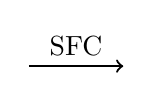
\begin{tikzpicture}[baseline={(current bounding box.center)}, scale=0.4]
            % Arrow from second grid to third grid
            \draw[->, thick] (0, 0) -- (3, 0)
            node[midway, above] {SFC};
        \end{tikzpicture}
        \hspace{2pt} % Decrease space here
        \begin{array}{|p{0.5cm}|p{0.5cm}|p{0.5cm}|p{0.5cm}|}
            \hline
             &   &   &   \\ \hline
             &   & A &   \\ \hline
             &   &   & A \\ \hline
             & 5 &   &   \\ \hline
        \end{array}
        \hspace{2pt} % Decrease space here
        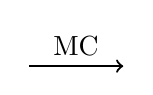
\begin{tikzpicture}[baseline={(current bounding box.center)}, scale=0.4]
            % Arrow from third grid to fourth grid
            \draw[->, thick] (0, 0) -- (3, 0)
            node[midway, above] {MC};
        \end{tikzpicture}
        \hspace{2pt} % Decrease space here
        \begin{array}{|p{0.5cm}|p{0.5cm}|p{0.5cm}|p{0.5cm}|}
            \hline
             & 5 & A & A \\ \hline
             & 5 &   & A \\ \hline
             & 5 & A &   \\ \hline
             &   & A & A \\ \hline
        \end{array}
        \)
        \hspace{2pt} % Decrease space here
        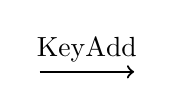
\begin{tikzpicture}[baseline={(current bounding box.center)}, scale=0.4]
            % Arrow from third grid to fourth grid
            \draw[->, thick] (0, 0) -- (3, 0)
            node[midway, above] {KeyAdd};
        \end{tikzpicture}

    }
\end{center}
\begin{center}
    \resizebox{\textwidth}{!}{%
        \(
        \begin{array}{|p{0.5cm}|p{0.5cm}|p{0.5cm}|p{0.5cm}|}
            \hline
             & 5 & A & A \\ \hline
             & 5 &   & A \\ \hline
             & 5 & A &   \\ \hline
             &   & A & A \\ \hline
        \end{array}
        \hspace{2pt} % Decrease space here
        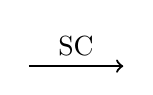
\begin{tikzpicture}[baseline={(current bounding box.center)}, scale=0.4]
            % Arrow from first grid to second grid
            \draw[->, thick] (0, 0) -- (3, 0)
            node[midway, above] {SC};
        \end{tikzpicture}
        \hspace{2pt} % Decrease space here
        \begin{array}{|p{0.5cm}|p{0.5cm}|p{0.5cm}|p{0.5cm}|}
            \hline
             & A & A & D \\ \hline
             & A &   & A \\ \hline
             & 7 & 5 &   \\ \hline
             &   & A & F \\ \hline
        \end{array}
        \hspace{2pt} % Decrease space here
        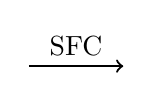
\begin{tikzpicture}[baseline={(current bounding box.center)}, scale=0.4]
            % Arrow from second grid to third grid
            \draw[->, thick] (0, 0) -- (3, 0)
            node[midway, above] {SFC};
        \end{tikzpicture}
        \hspace{2pt} % Decrease space here
        \begin{array}{|p{0.5cm}|p{0.5cm}|p{0.5cm}|p{0.5cm}|}
            \hline
              &   &   &   \\ \hline
            5 & A &   & A \\ \hline
            A & A & D &   \\ \hline
            F &   & 7 & A \\ \hline
        \end{array}
        \hspace{2pt} % Decrease space here
        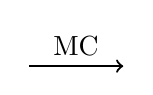
\begin{tikzpicture}[baseline={(current bounding box.center)}, scale=0.4]
            % Arrow from third grid to fourth grid
            \draw[->, thick] (0, 0) -- (3, 0)
            node[midway, above] {MC};
        \end{tikzpicture}
        \hspace{2pt} % Decrease space here
        \begin{array}{|p{0.5cm}|p{0.5cm}|p{0.5cm}|p{0.5cm}|}
            \hline
              &   & A &   \\ \hline
            5 & A & A & A \\ \hline
            A & A &   &   \\ \hline
            F &   & D & A \\ \hline
        \end{array}
        \)
        \hspace{2pt} % Decrease space here
        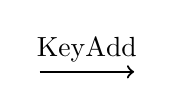
\begin{tikzpicture}[baseline={(current bounding box.center)}, scale=0.4]
            % Arrow from third grid to fourth grid
            \draw[->, thick] (0, 0) -- (3, 0)
            node[midway, above] {KeyAdd};
        \end{tikzpicture}

    }
\end{center}
\begin{center}
    \resizebox{\textwidth}{!}{%
        \(
        \begin{array}{|p{0.5cm}|p{0.5cm}|p{0.5cm}|p{0.5cm}|}
            \hline
              &   & A &   \\ \hline
            5 & A & A & A \\ \hline
            A & A & 7 &   \\ \hline
            F &   & D & A \\ \hline
        \end{array}
        \hspace{2pt} % Decrease space here
        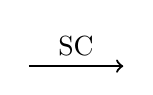
\begin{tikzpicture}[baseline={(current bounding box.center)}, scale=0.4]
            % Arrow from first grid to second grid
            \draw[->, thick] (0, 0) -- (3, 0)
            node[midway, above] {SC};
        \end{tikzpicture}
        \hspace{2pt} % Decrease space here
        \begin{array}{|p{0.5cm}|p{0.5cm}|p{0.5cm}|p{0.5cm}|}
            \hline
              &   & 5 &   \\ \hline
            7 & 5 & A & 5 \\ \hline
            5 & A & 5 &   \\ \hline
            A &   & 7 & 5 \\ \hline
        \end{array}
        \hspace{2pt} % Decrease space here
        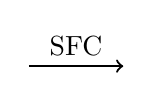
\begin{tikzpicture}[baseline={(current bounding box.center)}, scale=0.4]
            % Arrow from second grid to third grid
            \draw[->, thick] (0, 0) -- (3, 0)
            node[midway, above] {SFC};
        \end{tikzpicture}
        \hspace{2pt} % Decrease space here
        \begin{array}{|p{0.5cm}|p{0.5cm}|p{0.5cm}|p{0.5cm}|}
            \hline
              & A &   &   \\ \hline
            5 &   & A & 5 \\ \hline
            5 & 7 &   & 5 \\ \hline
            5 & 7 & A & 5 \\ \hline
        \end{array}
        \hspace{2pt} % Decrease space here
        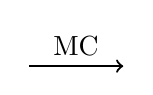
\begin{tikzpicture}[baseline={(current bounding box.center)}, scale=0.4]
            % Arrow from third grid to fourth grid
            \draw[->, thick] (0, 0) -- (3, 0)
            node[midway, above] {MC};
        \end{tikzpicture}
        \hspace{2pt} % Decrease space here
        \begin{array}{|p{0.5cm}|p{0.5cm}|p{0.5cm}|p{0.5cm}|}
            \hline
            5 &   &   & 5 \\ \hline
              &   &   &   \\ \hline
              & 7 & A &   \\ \hline
              & 7 &   &   \\ \hline
        \end{array}
        \)
        \hspace{2pt} % Decrease space here
        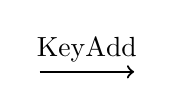
\begin{tikzpicture}[baseline={(current bounding box.center)}, scale=0.4]
            % Arrow from third grid to fourth grid
            \draw[->, thick] (0, 0) -- (3, 0)
            node[midway, above] {KeyAdd};
        \end{tikzpicture}
    }
\end{center}
\begin{center}
    \resizebox{\textwidth}{!}{%
        \(
        \begin{array}{|p{0.5cm}|p{0.5cm}|p{0.5cm}|p{0.5cm}|}
            \hline
            5 &   &   & 5 \\ \hline
              &   &   &   \\ \hline
              & 7 & A &   \\ \hline
              & 7 &   &   \\ \hline
        \end{array}
        \hspace{2pt} % Decrease space here
        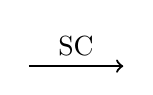
\begin{tikzpicture}[baseline={(current bounding box.center)}, scale=0.4]
            % Arrow from first grid to second grid
            \draw[->, thick] (0, 0) -- (3, 0)
            node[midway, above] {SC};
        \end{tikzpicture}
        \hspace{2pt} % Decrease space here
        \begin{array}{|p{0.5cm}|p{0.5cm}|p{0.5cm}|p{0.5cm}|}
            \hline
            A &   &   & A \\ \hline
              &   &   &   \\ \hline
              & 5 & A &   \\ \hline
              & 5 &   &   \\ \hline
        \end{array}
        \hspace{2pt} % Decrease space here
        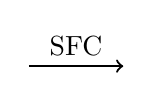
\begin{tikzpicture}[baseline={(current bounding box.center)}, scale=0.4]
            % Arrow from second grid to third grid
            \draw[->, thick] (0, 0) -- (3, 0)
            node[midway, above] {SFC};
        \end{tikzpicture}
        \hspace{2pt} % Decrease space here
        \begin{array}{|p{0.5cm}|p{0.5cm}|p{0.5cm}|p{0.5cm}|}
            \hline
            A &  &   & 5 \\ \hline
            A &  &   &   \\ \hline
              &  & A &   \\ \hline
              &  & 5 &   \\ \hline
        \end{array}
        \hspace{2pt} % Decrease space here
        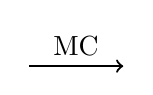
\begin{tikzpicture}[baseline={(current bounding box.center)}, scale=0.4]
            % Arrow from third grid to fourth grid
            \draw[->, thick] (0, 0) -- (3, 0)
            node[midway, above] {MC};
        \end{tikzpicture}
        \hspace{2pt} % Decrease space here
        \begin{array}{|p{0.5cm}|p{0.5cm}|p{0.5cm}|p{0.5cm}|}
            \hline
            A &  & F &   \\ \hline
            A &  & F & 5 \\ \hline
              &  & 5 & 5 \\ \hline
              &  & A & 5 \\ \hline
        \end{array}
        \hspace{2pt} % Decrease space here
        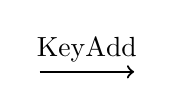
\begin{tikzpicture}[baseline={(current bounding box.center)}, scale=0.4]
            % Arrow from third grid to fourth grid
            \draw[->, thick] (0, 0) -- (3, 0)
            node[midway, above] {KeyAdd};
        \end{tikzpicture}
        \hspace{2pt} % Decrease space here
        \begin{array}{|p{0.5cm}|p{0.5cm}|p{0.5cm}|p{0.5cm}|}
            \hline
            A &  & F &   \\ \hline
            A &  & F & 5 \\ \hline
              &  & 5 & 5 \\ \hline
              &  & A & 5 \\ \hline
        \end{array}
        \)
    }

\end{center}
